\chapter{THIẾT KẾ CHI TIẾT}
    \section{Thiết kế chi tiết cơ khí}

        \subsection{Thiết kế thân robot}

            \hspace{0.5cm} Thân robot được thiết kế dạng tấm phẳng, đóng vai trò là kết cấu chính để gá lắp các cụm chân, động cơ servo, mạch điều khiển và pin. Kết cấu thân cần đảm bảo đủ độ cứng vững, hạn chế biến dạng trong quá trình robot di chuyển, đồng thời có khối lượng nhỏ để giảm tải cho các động cơ chân.

            \hspace{0.5cm} Các vị trí lắp servo được bố trí đối xứng hai bên thân robot nhằm đảm bảo phân bố tải trọng đều và giúp robot giữ cân bằng khi di chuyển. Các lỗ bắt vít servo, lỗ cố định mạch và pin phải được gia công đúng vị trí, đảm bảo lắp ráp dễ dàng, không bị lệch tâm hoặc gây kẹt cơ cấu chân.
            \begin{figure}[H]
                \centering
                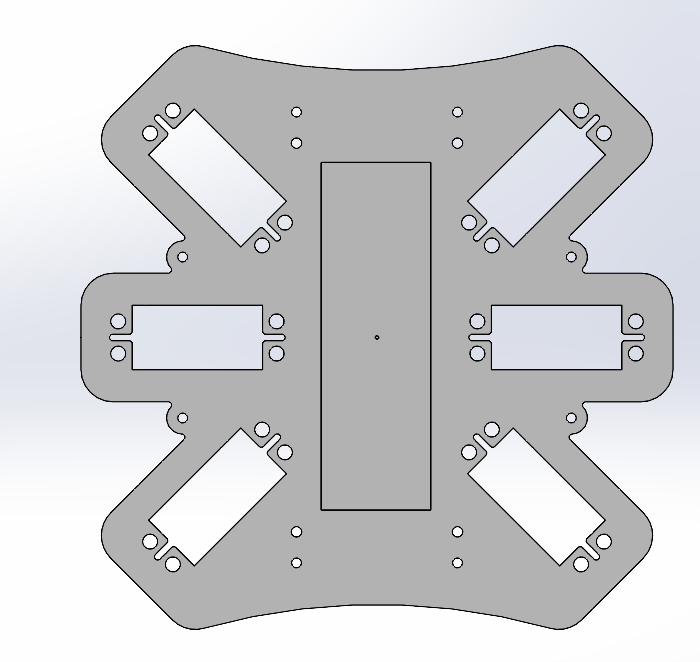
\includegraphics[width=0.5\textwidth]{pictures/robot_body.png}
                \caption{Thân robot}
            \end{figure}

        \subsection{Thiết kế cụm chân robot}

            \hspace{0.5cm} Phần chân của robot được chia thành 3 khớp bao gồm: khớp Coxa tương ứng với khớp háng, khớp Femur tương ứng với khớp đùi và khớp Tibia tương ứng với khớp chày của chân nhện.
            \subsubsection{Khớp Coxa}

            \hspace{0.5cm} Là khớp thứ nhất tương ứng với khớp háng, có tác dụng giúp các chân có thể dịch chuyển. Chất liệu được làm từ nhựa PLA. Các khớp Coxa ở phía trái và phải đối xứng nhau qua phần thân robot.

            \begin{figure}[H]
            \centering
            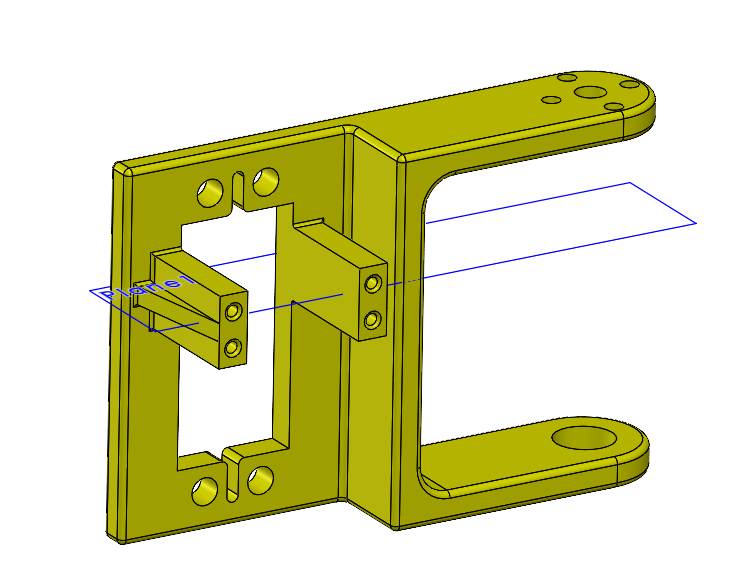
\includegraphics[width=0.5\textwidth]{pictures/coxa.png}
            \caption{Khớp Coxa}
            \end{figure}

            \subsubsection{Khớp Femur}

            \hspace{0.5cm} Là khớp thứ hai của robot, tương ứng với khớp đùi, có tác dụng là cầu nối giữa bộ phận khớp Tibia (khớp chày) và Coxa (khớp háng). Chất liệu khớp Femur được làm từ nhựa PLA. Khớp Femur được thiết kế theo dạng chữ H để tạo trục xoay cho đầu còn lại của servo. Mỗi đầu của khớp sẽ gắn với các đầu quay của servo để làm cầu nối.

            \begin{figure}[H]
            \centering
            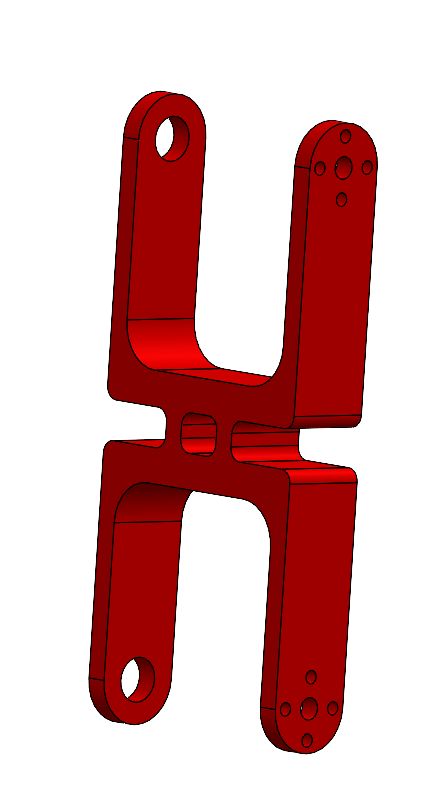
\includegraphics[width=0.25\textwidth]{pictures/femur.png}
            \caption{Khớp Femur}
            \end{figure}

            \subsubsection{Khớp Tibia}

            \hspace{0.5cm} Là khớp thứ ba của robot, tương ứng với khớp chày, tác dụng của khớp này giúp cho robot có thể đứng vững chắc. Khớp Tibia được làm từ chất liệu nhựa PLA. Các khớp Tibia ở phía trái và phía phải đối xứng nhau qua phần thân robot.

            \begin{figure}[H]
            \centering
            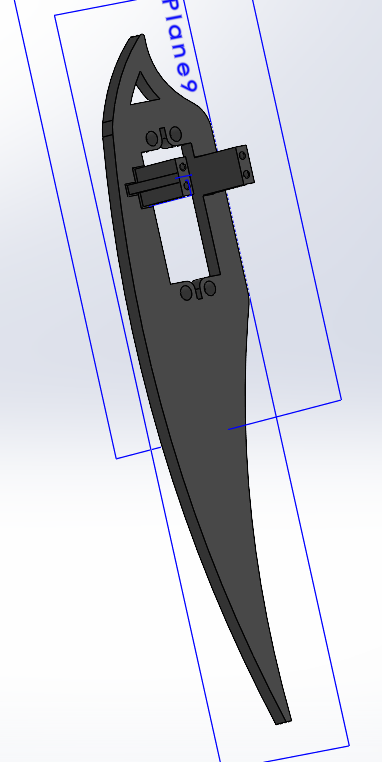
\includegraphics[width=0.25\textwidth]{pictures/tibia.png}
            \caption{Khớp Tibia}
            \end{figure}

        \subsection{Thông số cơ bản}

            \begin{table}[H]
            \centering
            \caption{Thông số cơ bản của robot}
            \begin{tabular}{|l|l|}
            \hline
            \textbf{Thông số} & \textbf{Giá trị} \\
            \hline
            Số chân & 6 \\
            \hline
            Kích thước chân L1--L2--L3 & 168--120--60 mm \\
            \hline
            Khối lượng robot & Xấp xỉ 2 kg \\
            \hline
            Vận tốc mong muốn & 0.5 m/s \\
            \hline
            \end{tabular}
            \end{table}

        \subsection{Tính toán lựa chọn động cơ}

            \hspace{0.5cm} Robot 6 chân có thể đạt ổn định tĩnh khi hình chiếu trọng tâm của robot nằm bên trong đa giác đỡ tạo bởi các chân đang tiếp xúc với mặt đất. Trong quá trình di chuyển với dáng đi tripod, tại một thời điểm thường có 3 chân tiếp xúc nền và 3 chân còn lại ở pha chuyển động. Đây là trường hợp bất lợi hơn so với trường hợp 5 chân tiếp xúc nền, vì tải trọng trung bình tác dụng lên mỗi chân lớn hơn. Do đó, tính toán lựa chọn động cơ được thực hiện theo trường hợp 3 chân tiếp xúc nền.

            \begin{figure}[H]
            \centering
            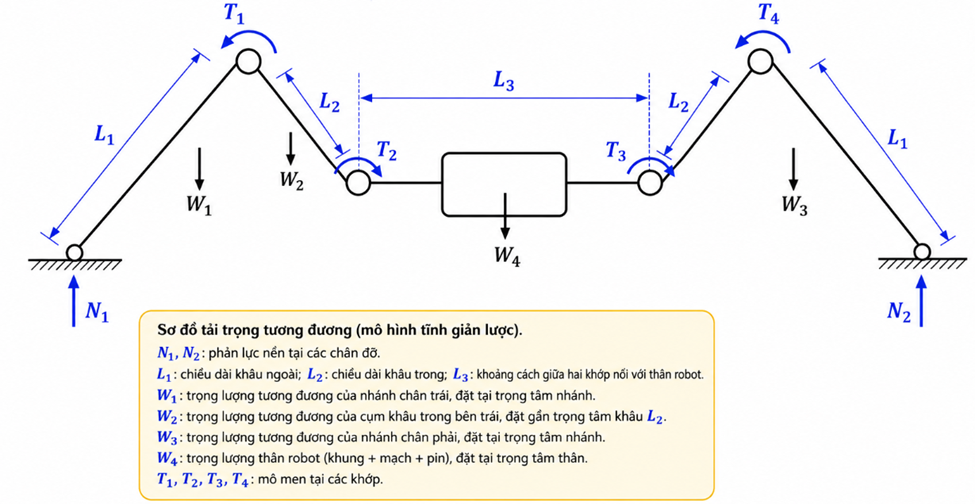
\includegraphics[width=0.7\textwidth]{pictures/load_model.png}
            \caption{Mô hình tải trọng tương đương của robot 6 chân}
            \end{figure}

            \subsubsection{Giả thiết tính toán}

            \hspace{0.5cm} Để đơn giản hóa bài toán và phù hợp với giai đoạn thiết kế sơ bộ, các giả thiết sau được sử dụng:
            \begin{itemize}
                \item Robot có khối lượng xấp xỉ $m = 2\;\text{kg}$.
                \item Tải trọng được giả thiết phân bố đều lên các chân đang tiếp xúc với mặt đất.
                \item Khối lượng của khung, mạch điện, pin, động cơ và các khâu chân được xét trong khối lượng tổng của robot. Ảnh hưởng của phân bố khối lượng thực tế, ma sát khớp và tải động được xét thông qua hệ số an toàn.
            \end{itemize}

            \hspace{0.5cm} Gia tốc trọng trường: $g = 9.81\;\text{m/s}^2$. Trọng lượng toàn bộ robot:
            \begin{equation}
                W = m \cdot g = 2 \times 9.81 = 19.62\;\text{N}
            \end{equation}

            \hspace{0.5cm} Các chiều dài khâu chân:
            \begin{equation}
                L_1 = 0.168\;\text{m}, \quad L_2 = 0.120\;\text{m}, \quad L_3 = 0.060\;\text{m}
            \end{equation}

            \subsubsection{Xác định phản lực tại chân}

            \hspace{0.5cm} Khi robot được đỡ bởi 3 chân, phản lực trung bình tại mỗi chân là:
            \begin{equation}
                N_3 = \frac{W}{3} = \frac{19.62}{3} = 6.54\;\text{N}
            \end{equation}

            \hspace{0.5cm} Khi robot được đỡ bởi 5 chân, phản lực trung bình tại mỗi chân là:
            \begin{equation}
                N_5 = \frac{W}{5} = \frac{19.62}{5} = 3.92\;\text{N}
            \end{equation}

            \hspace{0.5cm} Từ hai giá trị trên, trường hợp 3 chân tiếp xúc nền là trường hợp nguy hiểm hơn và được dùng làm cơ sở chính để lựa chọn động cơ.

            \subsubsection{Xác định mômen tại các khớp chân}

            \hspace{0.5cm} Trong mô hình phẳng tương đương, khi các khâu chân gần nằm ngang, mômen tại các khớp được tính theo tích lực và tay đòn. Với $N_3 = 6.54\;\text{N}$:
            \begin{equation}
                T_h = N_3 \times (L_1 + L_2 + L_3) = 6.54 \times 0.348 \approx 2.276\;\text{N.m} \approx 23.22\;\text{kgf.cm}
            \end{equation}
            \begin{equation}
                T_k = N_3 \times (L_2 + L_3) = 6.54 \times 0.180 \approx 1.177\;\text{N.m} \approx 12.00\;\text{kgf.cm}
            \end{equation}
            \begin{equation}
                T_d = N_3 \times L_3 = 6.54 \times 0.060 \approx 0.392\;\text{N.m} \approx 4.00\;\text{kgf.cm}
            \end{equation}

            \begin{table}[H]
            \centering
            \caption{Kết quả tính mômen tại các khớp chân}
            \begin{tabular}{|c|c|c|c|}
            \hline
            \textbf{Phản lực tại mỗi chân} & \boldmath$T_h$ & \boldmath$T_k$ & \boldmath$T_d$ \\
            \hline
            6.54 N & 23.22 kgf.cm & 12.00 kgf.cm & 4.00 kgf.cm \\
            \hline
            \end{tabular}
            \end{table}

            \subsubsection{Chọn hệ số an toàn và mômen yêu cầu}

            \hspace{0.5cm} Trong thực tế, mômen động cơ cần lớn hơn giá trị tính toán tĩnh do ma sát khớp, sai số lắp ráp, dao động khi chân tiếp xúc mặt đất và tải động. Chọn hệ số an toàn $K = 1.3$. Mômen yêu cầu đối với động cơ tại khớp chịu tải lớn nhất:
            \begin{equation}
                T_\text{cần} = K \times T_h = 1.3 \times 23.22 \approx 30.19\;\text{kgf.cm}
            \end{equation}

            \hspace{0.5cm} Do đó, động cơ được chọn cần thỏa mãn $T \geq 30.19\;\text{kgf.cm}$. Servo \textbf{MG996R} với mômen xoắn tối đa khoảng 13--15 kgf.cm ở 4.8--6V được chọn phù hợp cho các khớp chịu tải lớn nhất.

        \subsection{Kiểm nghiệm vận tốc}

            \hspace{0.5cm} Vận tốc di chuyển trung bình của robot phụ thuộc vào chiều dài bước và thời gian thực hiện một chu kỳ bước. Ngoài vận tốc trung bình, cần kiểm nghiệm thêm tốc độ quay yêu cầu của khớp hông để đảm bảo servo đáp ứng được yêu cầu động học.

            \begin{table}[H]
            \centering
            \caption{Thông số kiểm nghiệm vận tốc của robot}
            \begin{tabular}{|c|l|c|}
            \hline
            \textbf{Ký hiệu} & \textbf{Ý nghĩa} & \textbf{Giá trị} \\
            \hline
            $V_\text{mong muốn}$ & Vận tốc mong muốn của robot & 4 cm/s \\
            \hline
            $S$ & Chiều dài một bước & 30 mm = 3 cm \\
            \hline
            $T_{ck}$ & Thời gian một chu kỳ bước & 620 ms = 0.62 s \\
            \hline
            $\beta$ & Hệ số pha chống & 0.6 \\
            \hline
            $r$ & Bán kính quay tương đương khớp hông & 60 mm \\
            \hline
            \end{tabular}
            \end{table}

            \subsubsection{Kiểm nghiệm vận tốc trung bình}

            \hspace{0.5cm} Vận tốc trung bình của robot:
            \begin{equation}
                V = \frac{S}{T_{ck}} = \frac{3\;\text{cm}}{0.62\;\text{s}} \approx 4.84\;\text{cm/s}
            \end{equation}

            \hspace{0.5cm} Kết quả cho thấy vận tốc trung bình đạt khoảng $4.84\;\text{cm/s}$, phù hợp với yêu cầu vận tốc 4 cm/s. Tần số bước tương ứng là:
            \begin{equation}
                f = \frac{1}{T_{ck}} = \frac{1}{0.62} \approx 1.61\;\text{Hz}
            \end{equation}

            \subsubsection{Kiểm nghiệm góc quay khớp hông}

            \hspace{0.5cm} Giả sử chuyển động tạo bước chủ yếu được thực hiện bởi chuyển động quay của khớp hông. Chiều dài bước được xấp xỉ theo quan hệ hình học $S = 2r\sin(\alpha)$, từ đó:
            \begin{equation}
                \alpha = \arcsin\!\left(\frac{S}{2r}\right) = \arcsin\!\left(\frac{30}{2 \times 60}\right) = \arcsin(0.25) \approx 14.5°
            \end{equation}

            \hspace{0.5cm} Góc quay tổng trong pha vung (cả hai phía): $\alpha_\text{tổng} = 2\alpha \approx 29°$.

            \subsubsection{Kiểm nghiệm tốc độ quay yêu cầu của servo hông}

            \hspace{0.5cm} Thời gian pha vung chân: $t_\text{vung} = (1 - \beta) \cdot T_{ck} = 0.4 \times 0.62 = 0.248\;\text{s}$

            \hspace{0.5cm} Tốc độ góc yêu cầu của servo:
            \begin{equation}
                \omega = \frac{\alpha_\text{tổng}}{t_\text{vung}} = \frac{29°}{0.248\;\text{s}} \approx 116.9°/\text{s}
            \end{equation}

            \hspace{0.5cm} Thời gian quay $60°$ tương đương:
            \begin{equation}
                t_{60} = \frac{60°}{116.9°/\text{s}} \approx 0.51\;\text{s}/60°
            \end{equation}

            \hspace{0.5cm} Servo MG996R có tốc độ $0.17\;\text{s}/60°$ (ở 6V), nhỏ hơn $0.51\;\text{s}/60°$, do đó servo đáp ứng yêu cầu về tốc độ quay để robot đạt vận tốc thiết kế.

        \subsection{Phân tích lực bằng ANSYS}

            \hspace{0.5cm} Để kiểm tra độ bền kết cấu, mô phỏng tĩnh được thực hiện trên toàn bộ mô hình robot bằng phần mềm ANSYS.

            \subsubsection{Kết quả ứng suất (Stress)}

            \begin{figure}[H]
            \centering
            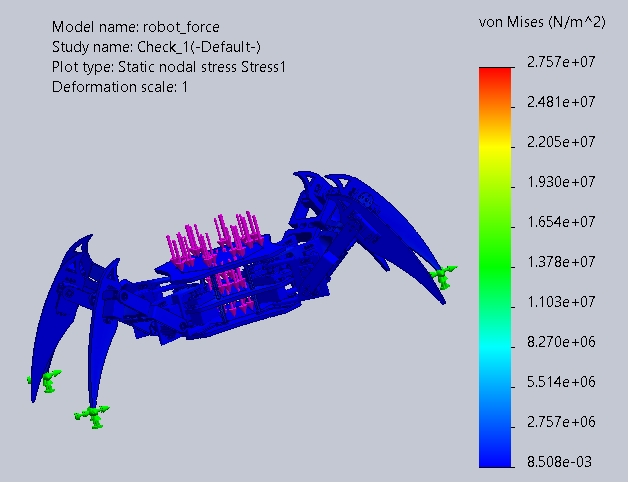
\includegraphics[width=0.85\textwidth]{pictures/solidsolid_stress.png}
            \caption{Kết quả ứng suất von Mises (Stress)}
            \end{figure}

            \hspace{0.5cm} Kết quả mô phỏng tĩnh cho thấy ứng suất von Mises lớn nhất tập trung cục bộ tại một số vị trí liên kết, lỗ bắt vít hoặc vùng gần điểm chịu tải. Phần lớn kết cấu có màu xanh, chứng tỏ ứng suất phân bố trên thân robot tương đối nhỏ. Với mức ứng suất này, thân robot có khả năng chịu tải tốt trong điều kiện mô phỏng tĩnh.

            \subsubsection{Kết quả chuyển vị (Displacement)}
            \begin{figure}[H]
            \centering
            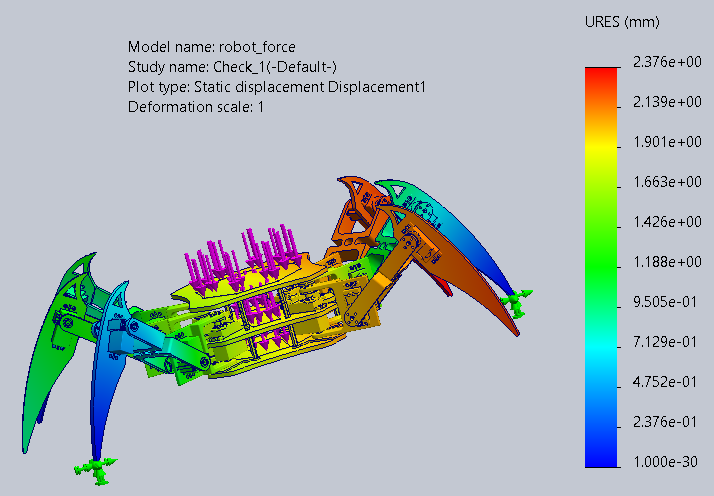
\includegraphics[width=0.85\textwidth]{pictures/solidworks_displacement.png}
            \caption{Kết quả chuyển vị (Displacement)}
            \end{figure}

            \hspace{0.5cm} Kết quả phân tích chuyển vị tĩnh cho thấy chuyển vị tổng lớn nhất của robot đạt khoảng $2.376\;\text{mm}$. Chuyển vị tập trung chủ yếu tại các đầu chân và các vùng xa vị trí liên kết cố định do ảnh hưởng của tay đòn lớn. Phần thân trung tâm có mức chuyển vị nhỏ hơn, chứng tỏ kết cấu thân robot có độ cứng vững tương đối tốt. Giá trị chuyển vị này cần được xem xét để đảm bảo khe hở lắp ráp và hành trình chuyển động của chân đủ lớn, tránh va chạm trong quá trình hoạt động.

            \subsubsection{Kết quả biến dạng tương đương (Strain)}

            \begin{figure}[H]
            \centering
            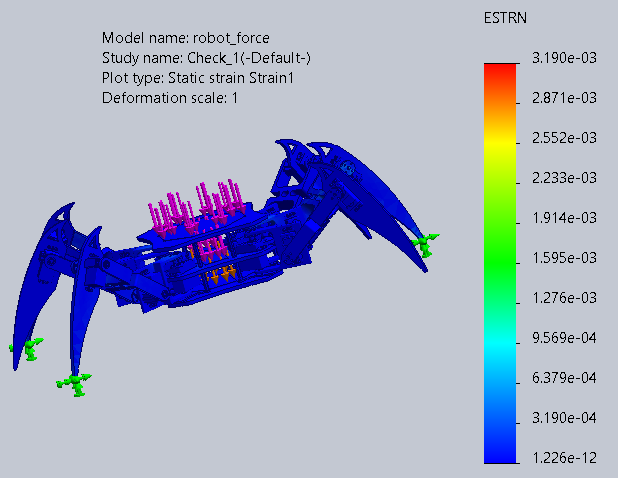
\includegraphics[width=0.85\textwidth]{pictures/solidsolid_strain.png}
            \caption{Kết quả biến dạng tương đương (Strain)}
            \end{figure}

            \hspace{0.5cm} Kết quả mô phỏng biến dạng cho thấy biến dạng tương đương lớn nhất của robot là $\varepsilon_\text{max} = 3.19 \times 10^{-3}$, tương đương khoảng 0.319\%. Phần lớn kết cấu có biến dạng nhỏ, chỉ tập trung cục bộ tại các vùng liên kết và vị trí bắt vít. Điều này phù hợp với kết quả ứng suất và chuyển vị trước đó, xác nhận rằng kết cấu tổng thể của robot có đủ độ cứng vững trong điều kiện tải trọng mô phỏng.

    \section{Thiết kế chi tiết điện}
        \subsection{Thông số linh kiện}

            \subsubsection{Servo MG996R}

            \begin{table}[H]
            \centering
            \caption{Thông số kỹ thuật servo MG996R}
            \label{tab:mg996r_specs}
            \begin{tabular}{|>{\raggedright\arraybackslash}m{7cm}|>{\centering\arraybackslash}m{7cm}|}
            \hline
            \textbf{Thông số} & \textbf{Giá trị} \\
            \hline
            Mô-men xoắn cực đại (Stall torque) & 9.4 kgf·cm (4.8V) / 11 kgf·cm (6V) \\
            \hline
            Tốc độ hoạt động (Operating speed) & 0.17 s/60° (4.8V) / 0.14 s/60° (6V) \\
            \hline
            Điện áp hoạt động (Operating voltage) & 4.8 -- 7.2 V \\
            \hline
            Dòng khi hoạt động (Running current) & 500 -- 900 mA \\
            \hline
            Dòng khi kẹt (Stall current) & 2.5 A (6V) \\
            \hline
            Độ rộng vùng chết (Dead band width) & 5 $\mu$s \\
            \hline
            Thiết kế & Ổn định, chống rung với ổ bi kép (double ball bearing) \\
            \hline
            Khối lượng (Weight) & 55 g \\
            \hline
            Kích thước (Dimension) & 40.7 $\times$ 19.7 $\times$ 42.9 mm \\
            \hline
            Số lượng & 18 \\
            \hline
            \end{tabular}
            \end{table}

            \subsubsection{ESP32 WROOM-32}

            \begin{table}[H]
            \centering
            \caption{Thông số kỹ thuật ESP32 WROOM-32}
            \label{tab:esp32_specs}
            \begin{tabular}{|>{\raggedright\arraybackslash}m{7cm}|>{\centering\arraybackslash}m{7cm}|}
            \hline
            \textbf{Thông số} & \textbf{Giá trị} \\
            \hline
            Thạch anh tích hợp & 40 MHz \\
            \hline
            Bộ nhớ Flash SPI tích hợp & 4 MB \\
            \hline
            Điện áp cấp & 5 V \\
            \hline
            Dòng điện cấp & 500 mA \\
            \hline
            Dòng khi hoạt động & 80 mA \\
            \hline
            \end{tabular}
            \end{table}

            \subsubsection{PCA9685}

            \begin{table}[H]
            \centering
            \caption{Thông số kỹ thuật PCA9685}
            \label{tab:pca9685_specs}
            \begin{tabular}{|>{\raggedright\arraybackslash}m{7cm}|>{\centering\arraybackslash}m{7cm}|}
            \hline
            \textbf{Thông số} & \textbf{Giá trị} \\
            \hline
            Điện áp cấp & 2.3 -- 5.5 V \\
            \hline
            Dòng điện cấp & 6 -- 10 mA \\
            \hline
            Dòng điện tối đa & 25 mA \\
            \hline
            \end{tabular}
            \end{table}

            \subsubsection{HY-SRF05}

            \begin{table}[H]
            \centering
            \caption{Thông số kỹ thuật cảm biến siêu âm HY-SRF05}
            \label{tab:srf05_specs}
            \begin{tabular}{|>{\raggedright\arraybackslash}m{7cm}|>{\centering\arraybackslash}m{7cm}|}
            \hline
            \textbf{Thông số} & \textbf{Giá trị} \\
            \hline
            Điện áp hoạt động & 5 V \\
            \hline
            Dòng điện tĩnh & \ldots \\
            \hline
            \end{tabular}
            \end{table}

        \subsection{Thiết kế nguồn động lực}

        \hspace{0.5cm} Dòng điện tiêu thụ của 18 servo ở chế độ hoạt động:
        \begin{equation}
            I_{\text{servo}} = 18 \times 900\text{ mA} = 16.2\text{ A}
        \end{equation}

        Chọn hệ số an toàn $SF = 1.5$, dòng điện thiết kế:
        \begin{equation}
            I_{\text{tk}} = SF \times I_{\text{servo}} = 24.3 \text{ A}
        \end{equation}

        Do trong thực tế không có trường hợp tất cả servo cùng hoạt động với tải tối đa cùng lúc nên thiết kế nguồn có $I_{\text{tk}} = 24.3 (A)$ là quá đủ cho robot.

        Điện áp hoạt động của servo là 4.8 -- 7.2 V nên chọn nguồn là pin LiPo 3S (11.1 V) kết hợp buck converter. Không dùng LiPo 2S do điện áp danh định 7.4 V vượt mức cho phép của servo; ngoài ra khi qua buck converter sẽ không đảm bảo dòng đầu ra ổn định.

        Chọn IC buck converter \textbf{XL4016E} với các thông số kỹ thuật trình bày trong Bảng~\ref{tab:xl4016e_specs}:

        \begin{table}[H]
        \centering
        \caption{Thông số kỹ thuật IC buck converter XL4016E}
        \label{tab:xl4016e_specs}
        \begin{tabular}{|>{\raggedright\arraybackslash}m{7cm}|>{\centering\arraybackslash}m{7cm}|}
        \hline
        \textbf{Thông số} & \textbf{Giá trị} \\
        \hline
        Điện áp ngõ vào tối thiểu & 8 V \\
        \hline
        Điện áp ngõ vào tối đa & 40 V \\
        \hline
        Dòng điện ngõ ra & 8 A \\
        \hline
        Nhiệt độ hoạt động & -40 -- 80 \textdegree C \\
        \hline
        \end{tabular}
        \end{table}

        Do dòng điện ngõ ra tối đa của mỗi XL4016E là 8 A, trong khi mỗi nhóm 6 servo có thể tiêu thụ tới $6 \times 900\text{ mA} = 5.4\text{ A}$ ở chế độ hoạt động, nên sử dụng \textbf{3 bộ buck converter}, mỗi bộ cấp nguồn cho 6 servo, đảm bảo dòng đầu ra đủ đáp ứng toàn bộ hệ thống.tử
        \begin{figure}[H]
            \centering
            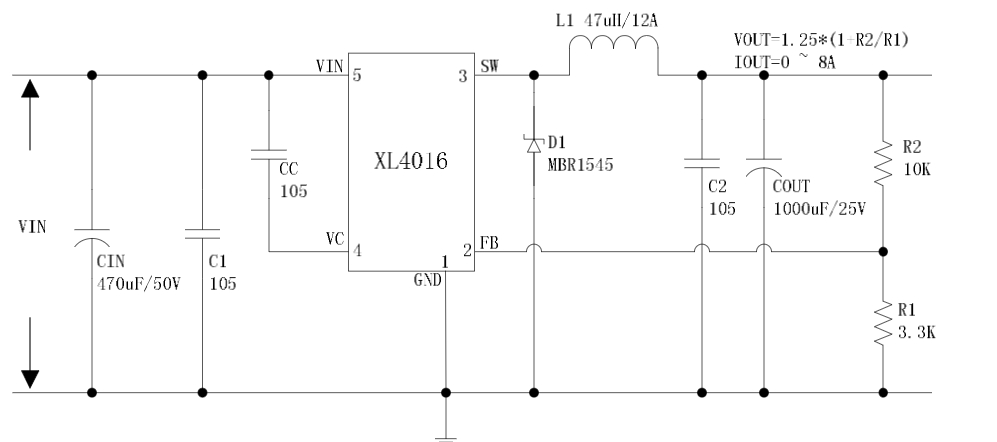
\includegraphics[width=0.8\textwidth]{pictures/XL4016E.png}
            \caption{Buck Converter XL4016E}
            \label{fig:power_distribution}
        \end{figure}
        \begin{figure}[H]
            \centering
            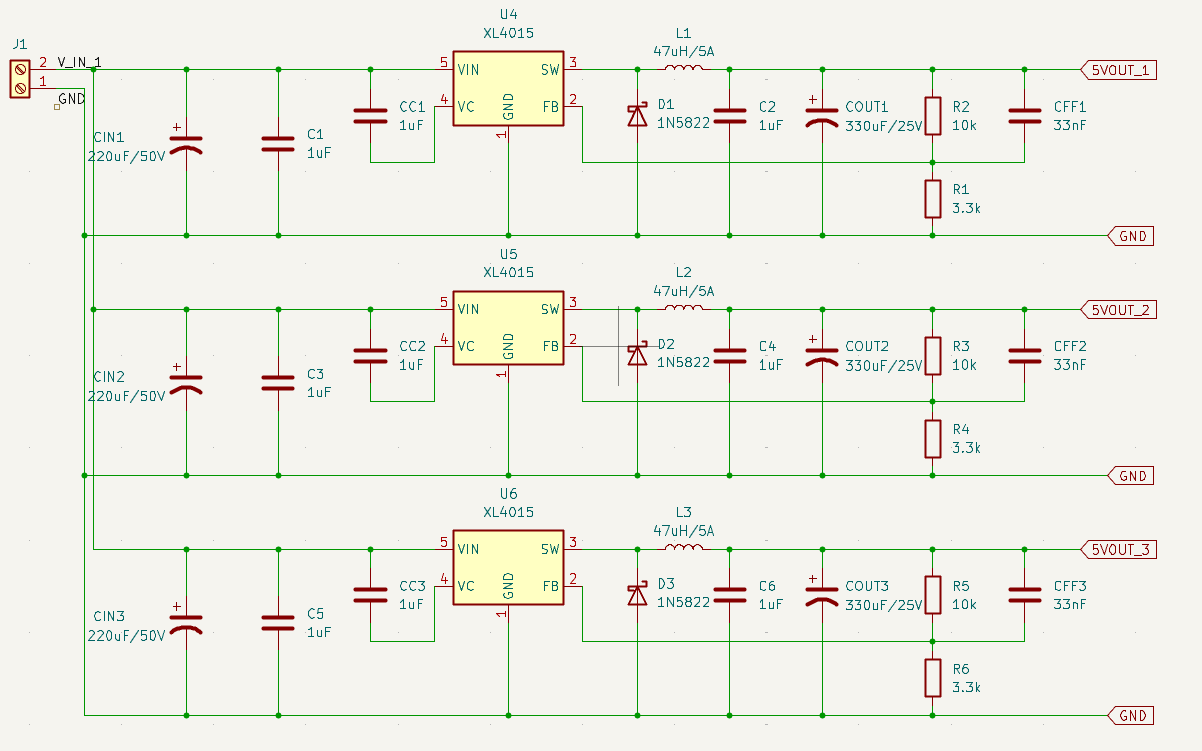
\includegraphics[width=1\textwidth]{pictures/DynamicPowerSource.png}
            \caption{Schematic mạch nguồn động lực}
            \label{fig:control_circuit_diagram}
        \end{figure}
        \subsection{Thiết kế nguồn điều khiển}
        \hspace{0.5cm} Dòng điện tiêu thụ của ESP32 WROOM-32 là 80 mA, dòng điện tiêu thụ của mỗi PCA9685 là 10 mA còn dòng tiêu thụ của cảm biến siêu âm là 20 mA, tổng dòng điện tiêu thụ của mạch điều khiển:
        \begin{equation}
            I_{\text{control}} = 80\text{ mA} + 2 \times 10\text{ mA} + 20\text{ mA} = 120\text{ mA}
        \end{equation}
        \hspace*{0.5cm} Chọn nguồn mạch điều khiển là nguồn 2 pin Lithium 3.7V và Buck converter là LM2596S-5.0 5V 3A.
        \begin{figure}[H]
            \centering
            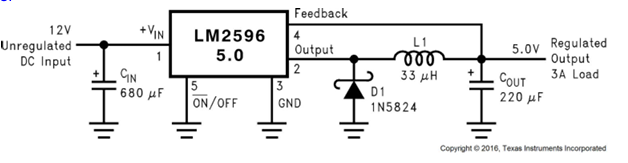
\includegraphics[width=0.8\textwidth]{pictures/Lm2596S-5.0.png}
            \caption{Buck Converter Lm2596S-5.0}
            \label{fig:control_circuit}
        \end{figure}
         \begin{figure}[H]
            \centering
            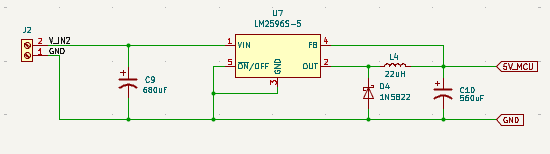
\includegraphics[width=1\textwidth]{pictures/ControlPowerSource.png}
            \caption{Schematic mạch nguồn điều khiển}
            \label{fig:control_circuit_diagram}
        \end{figure}
        \subsection{Thiết kế mạch điều khiển}
        \begin{itemize}
            \item Sử dụng 2 IC PCA9685 để điều khiển 18 servo, mỗi IC điều khiển 9 servo.
            \item ESP32 WROOM-32 giao tiếp với các PCA9685 qua giao thức I2C, sử dụng địa chỉ I2C khác nhau cho mỗi IC.
            \item Cảm biến siêu âm HY-SRF05 được kết nối với ESP32 để thu thập dữ liệu khoảng cách, hỗ trợ chức năng tránh vật cản.

        \end{itemize}
        
        
       
        \begin{figure}[H]
            \centering
            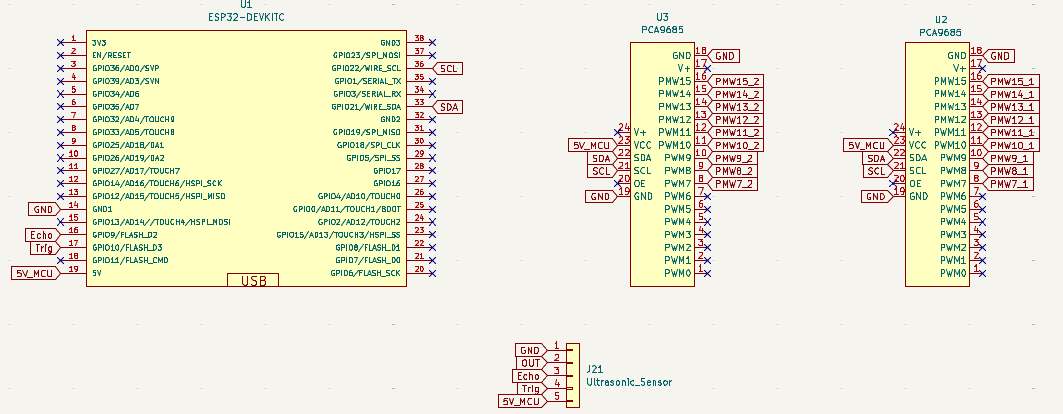
\includegraphics[width=1\textwidth]{pictures/ControlSchematic}
            \caption{Schematic mạch điều khiển}
            \label{fig:control_circuit_diagram}
        \end{figure}
        \begin{figure}[H]
            \centering
            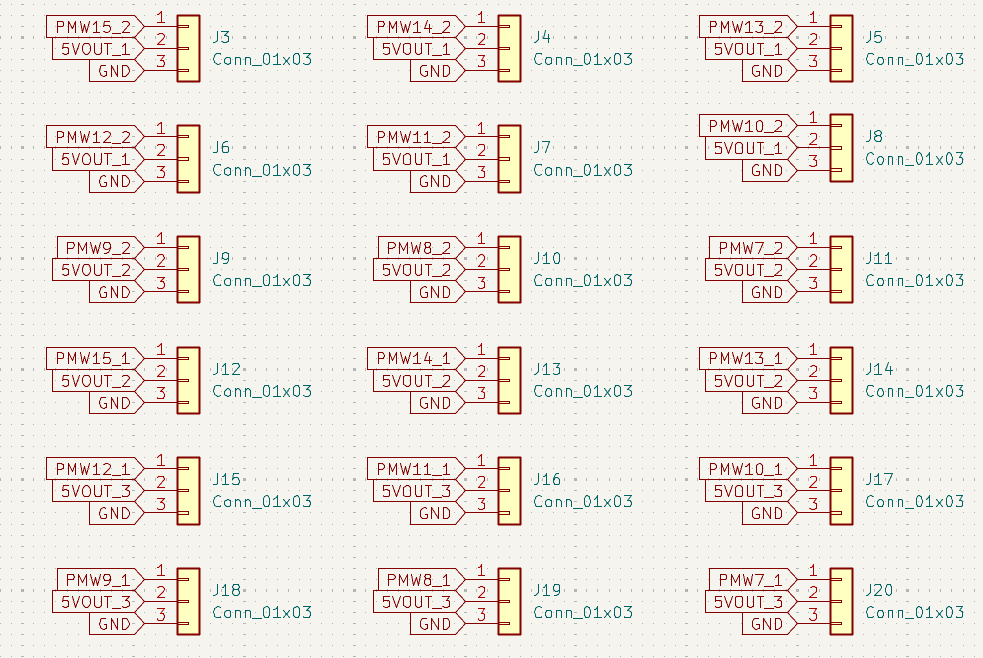
\includegraphics[width=1\textwidth]{pictures/Header}
            \caption{Schematic header kết nối giữa các module}
            \label{fig:control_circuit_diagram}
        \end{figure}
        \subsection{Thiết kế mạch in PCB}
        \hspace{0.5cm} Mạch in PCB được thiết kế để tích hợp các thành phần điện tử, đảm bảo kết nối ổn định và hiệu quả giữa các module. \\
        \hspace*{0.5cm} Mạch in sử dụng 2 lớp, lớp trên được dùng cho việc bố trí linh kiện và đi dây nguồn, lớp dưới được dùng cho việc đi dây tín hiệu, cả 2 lớp đều được phủ GND. Các linh kiện được bố trí hợp lý để giảm thiểu chiều dài đường dẫn và tránh nhiễu điện từ. \\
        \begin{figure}[H]
            \centering
            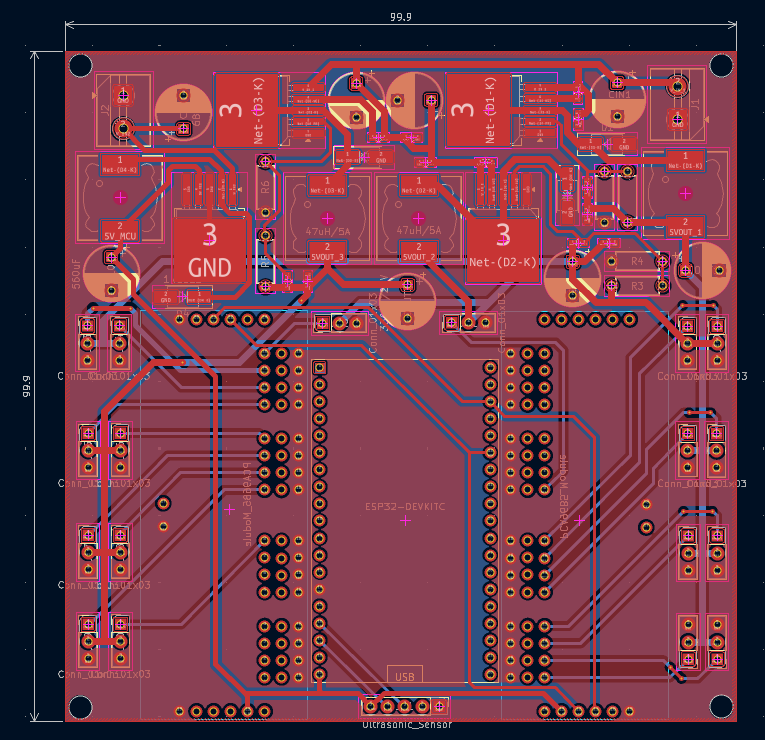
\includegraphics[width=0.7\textwidth]{pictures/PCBLayout.png}
            \caption{Layout mạch in PCB}
            \label{fig:pcb_layout}
        \end{figure}
        \begin{figure}[H]
            \centering
            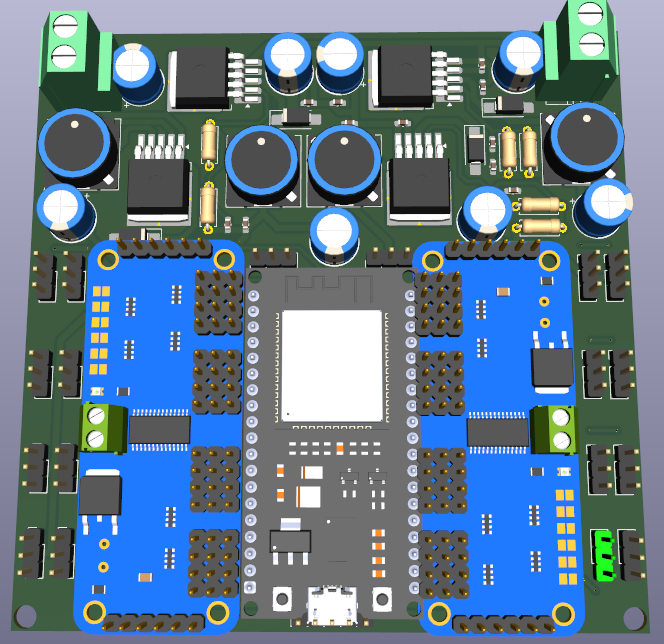
\includegraphics[width=0.7\textwidth]{pictures/PCB3D.png}
            \caption{Mô hình 3D mạch in PCB}
            \label{fig:pcb_3D}
        \end{figure}
    \section{Thiết kế chi tiết giải thuật điều khiển}

        \subsection{Chuyển đổi hệ tọa độ}

        \hspace{0.5cm} Tọa độ đầu chân trong firmware được biểu diễn theo \textbf{hệ tọa độ thân robot} (body frame). Trước khi gọi IK, cần chuyển sang \textbf{hệ tọa độ chân} (leg frame) bằng phép quay ngược chiều góc gắn chân $\psi_i$:

        \begin{equation}
            \begin{bmatrix} l_x \\ l_y \end{bmatrix}
            =
            \begin{bmatrix} \cos\psi_i & \sin\psi_i \\ -\sin\psi_i & \cos\psi_i \end{bmatrix}
            \begin{bmatrix} x \\ y \end{bmatrix}
        \end{equation}

        trong đó $\psi_i$ là góc gắn chân thứ $i$ đo từ trục $X$ thân robot (LF: $45°$, LM: $90°$, LB: $135°$, RF: $-45°$, RM: $-90°$, RB: $-135°$). Tọa độ $z$ không thay đổi qua phép chiếu này.

        \subsection{Giải thuật động học nghịch}

        \hspace{0.5cm} Sau khi có tọa độ $(l_x, l_y, z)$ trong leg frame, giải IK bằng phương pháp hình học:

        \textbf{Bước 1 — Góc coxa:}
        \begin{equation}
            \theta_1 = \mathrm{atan2}(l_y,\, l_x)
        \end{equation}

        \textbf{Bước 2 — Khoảng cách nằm ngang từ gốc femur đến đầu chân:}
        \begin{equation}
            d = \sqrt{l_x^2 + l_y^2} - L_1
        \end{equation}

        \textbf{Bước 3 — Độ dài đường chéo femur–đầu chân:}
        \begin{equation}
            D = \sqrt{d^2 + z^2}
        \end{equation}

        Điều kiện vùng làm việc: $|L_2 - L_3| \leq D \leq L_2 + L_3$. Nếu không thỏa, trả về \texttt{valid = false} và servo giữ nguyên vị trí.

        \textbf{Bước 4 — Góc tibia (định lý cosin):}
        \begin{equation}
            \cos\theta_3 = \frac{D^2 - L_2^2 - L_3^2}{2\,L_2 L_3}, \qquad \theta_3 = \arccos(\cos\theta_3)
        \end{equation}

        \textbf{Bước 5 — Góc femur:}
        \begin{equation}
            \theta_2 = \mathrm{atan2}(z,\, d) - \mathrm{atan2}\!\left(L_3\sin\theta_3,\; L_2 + L_3\cos\theta_3\right)
        \end{equation}

        Cấu hình elbow-down được chọn (dấu $+$ trong $\theta_3$) để đảm bảo khoảng tĩnh không dưới thân robot.

        \subsection{Chuyển đổi góc sang PWM}

        \hspace{0.5cm} Góc khớp (độ) được chuyển sang độ rộng xung PWM theo công thức tuyến tính. PCA9685 hoạt động ở 50 Hz với bộ đếm 12-bit (4096 tick). Với servo MG996R có dải xung 0.5 ms -- 2.5 ms:

        \begin{equation}
            \text{tick}_{\min} = \left\lfloor 0.5 \times 10^{-3} \times 50 \times 4096 \right\rfloor = 102
        \end{equation}
        \begin{equation}
            \text{tick}_{\max} = \left\lfloor 2.5 \times 10^{-3} \times 50 \times 4096 \right\rfloor = 512
        \end{equation}
        \begin{equation}
            \text{tick}(\theta) = 102 + \frac{\theta}{180^\circ} \times 410
        \end{equation}

        \subsection{Giải thuật dáng đi Tripod}

        \hspace{0.5cm} Robot sử dụng dáng đi tripod với 6 chân chia thành hai nhóm:
        \begin{itemize}
            \item \textbf{Nhóm A:} LF, RM, LB — phase 0
            \item \textbf{Nhóm B:} RF, LM, RB — phase 0.5 
        \end{itemize}

        Mỗi chu kỳ gait gồm hai nửa bước đối xứng. Sau Tripod Init thì nhện có tư thế đứng, yên nhóm A ở BWD, nhóm B ở FWD. Bảng~\ref{tab:tripod_timing} trình bày chuỗi sự kiện và thời gian tương ứng:

        \begin{table}[H]
        \centering
        \caption{Chuỗi sự kiện một chu kỳ tripod gait}
        \label{tab:tripod_timing}
        \begin{tabular}{|c|l|c|l|}
        \hline
        \textbf{Pha} & \textbf{Sự kiện} & \textbf{Thời gian (ms)} & \textbf{Nhóm stance di chuyển} \\
        \hline
        \multirow{4}{*}{Nửa bước 1} & Stance (B) về neutral & 80 & $+\mathtt{step\_x}$ mm \\
        & Swing (A): nhấc lên & 120 ($T_\mathrm{lift}$) & đứng yên \\
        & Swing (A): đưa ra trước & 220 ($T_\mathrm{swing}$) & đứng yên \\
        & Swing (A): hạ xuống & 120 ($T_\mathrm{down}$) & đứng yên \\
        & Stance (B) về BWD & 80 & $+\mathtt{step\_x}$ mm \\
        \hline
        \multirow{4}{*}{Nửa bước 2} & Stance (A) về neutral & 80 & $+\mathtt{step\_x}$ mm \\
        & Swing (B): nhấc lên & 120 ($T_\mathrm{lift}$) & đứng yên \\
        & Swing (B): đưa ra trước & 220 ($T_\mathrm{swing}$) & đứng yên \\
        & Swing (B): hạ xuống & 120 ($T_\mathrm{down}$) & đứng yên \\
        & Stance (A) về BWD & 80 & $+\mathtt{step\_x}$ mm \\
        \hline
        \multicolumn{2}{|l|}{\textbf{Tổng 1 chu kỳ}} & \textbf{1240 ms} & $4 \times \mathtt{step\_x}$ mm \\
        \hline
        \end{tabular}
        \end{table}

        \hspace{0.5cm} Thân robot chỉ tiến trong bốn đoạn 80 ms (stance di chuyển), còn lại đứng yên trong khi nhóm swing đang bay. Vận tốc tịnh tiến:

        \begin{equation}
            v = \frac{4 \times \mathtt{step\_x}}{2 \times (160 + T_\mathrm{lift} + T_\mathrm{swing} + T_\mathrm{down})}
        \end{equation}

        Với tham số mặc định ($\mathtt{step\_x} = 15$ mm, $T_\mathrm{lift} = T_\mathrm{down} = 120$ ms, $T_\mathrm{swing} = 220$ ms):
        \begin{equation}
            v = \frac{4 \times 15}{2 \times (160 + 120 + 220 + 120)} = \frac{60}{1240} \approx 4.8 \text{ cm/s}
        \end{equation}

        \subsection{State machine tránh vật cản}

        \hspace{0.5cm} Giải thuật tránh vật cản được cài đặt như một state machine hai trạng thái, chạy trước mỗi lần gọi \texttt{tripod\_step()}:

        \begin{table}[H]
        \centering
        \caption{State machine tránh vật cản}
        \label{tab:obs_sm}
        \begin{tabular}{|l|l|l|l|}
        \hline
        \textbf{Trạng thái} & \textbf{Điều kiện} & \textbf{Hành động} & \textbf{Chuyển sang} \\
        \hline
        \multirow{4}{*}{NORMAL} & $d < 0$ (lỗi sensor) & \texttt{trim\_y = 0} (thẳng) & NORMAL \\
        & $d < 12$ cm & \texttt{trim\_y = 18} mm, đếm 6 bước & TURNING \\
        & $12 \leq d < 25$ cm & \texttt{trim\_y = 4} mm (lệch nhẹ) & NORMAL \\
        & $d \geq 25$ cm & \texttt{trim\_y = 0} (thẳng) & NORMAL \\
        \hline
        TURNING & đếm xuống = 0 & \texttt{trim\_y = 0}, reset & NORMAL \\
        \hline
        \end{tabular}
        \end{table}

        Tham số \texttt{trim\_y} được đưa vào hàm \texttt{gait\_set\_params()} và áp dụng ngay cho bước tiếp theo. Lệch phải tương ứng \texttt{trim\_y} $> 0$ (tọa độ $y$ của FWD giảm, BWD tăng trên tất cả các chân). Sau 6 bước quay ($\approx 6 \times 1240 = 7440$ ms $\approx 90°$), robot tự động quay lại chế độ NORMAL và tiếp tục đi thẳng.

    \section{Thiết kế chi tiết phần mềm}

        \subsection{Cấu trúc module}

        \hspace{0.5cm} Web app được tổ chức theo cấu trúc module như Bảng~\ref{tab:webapp_modules}:

        \begin{table}[H]
        \centering
        \caption{Cấu trúc module web app}
        \label{tab:webapp_modules}
        \begin{tabular}{|>{\centering\arraybackslash}m{8cm}|>{\centering\arraybackslash}m{8cm}|}
        \hline
        \textbf{File / Module} & \textbf{Chức năng} \\
        \hline
        \texttt{context/WsContext.jsx} & Quản lý WebSocket, ping-pong latency, broadcast state \\
        \texttt{context/RobotContext.jsx} & State toàn cục robot, RAF animation, đồng bộ firmware \\
        \texttt{utils/kinematics.js} & IK, FK, bodyToLegFrame (mirror firmware) \\
        \texttt{constants/robotConfig.js} & Hằng số vật lý robot (L1, L2, L3, STAND\_Z, ...) \\
        \texttt{components/layout/TopBar.jsx} & Kết nối WS, Start/Stop, hiển thị latency, dist, speed \\
        \texttt{components/settings/SettingsPanel.jsx} & Slider offset servo, tham số gait, pose mode \\
        \texttt{components/viewer/SpiderViewer.jsx} & Render 3D robot (React Three Fiber) \\
        \texttt{components/layout/AngleDisplay.jsx} & Bảng góc khớp số thời gian thực \\
        \hline
        \end{tabular}
        \end{table}

        \subsection{Giao thức WebSocket chi tiết}

        \hspace{0.5cm} Bảng~\ref{tab:ws_protocol} liệt kê toàn bộ bản tin JSON trong giao thức WebSocket giữa web app và firmware:

        \begin{table}[H]
        \centering
        \caption{Giao thức WebSocket}
        \label{tab:ws_protocol}
        \begin{tabular}{|>{\centering\arraybackslash}m{4cm}|>{\centering\arraybackslash}m{4cm}|>{\centering\arraybackslash}m{7cm}|}
        \hline
        \textbf{Hướng} & \textbf{Bản tin (cmd)} & \textbf{Tham số / Mô tả} \\
        \hline
        App $\to$ ESP32 & \texttt{start} & Bắt đầu tripod gait, kèm \texttt{gait} params \\
        App $\to$ ESP32 & \texttt{stop} & Dừng gait, về tư thế đứng \\
        App $\to$ ESP32 & \texttt{set\_height} & \texttt{z}: chiều cao thân (mm) \\
        App $\to$ ESP32 & \texttt{set\_gait} & \texttt{stepX, liftZ, tLiftMs, tSwingMs, tDownMs, trimY} \\
        App $\to$ ESP32 & \texttt{set\_offset} & \texttt{leg, cx, fm, tb}: offset góc servo (độ) \\
        App $\to$ ESP32 & \texttt{set\_foot} & \texttt{leg, x, y, z}: tọa độ đầu chân (pose mode) \\
        App $\to$ ESP32 & \texttt{ping} & Đo latency (gửi mỗi 2 giây) \\
        \hline
        ESP32 $\to$ App & \texttt{pong} & Phản hồi ping, app tính latency \\
        ESP32 $\to$ App & \texttt{\{"dist\_cm": ...\/\}} & Khoảng cách SRF05 (cm), broadcast mỗi bước gait \\
        ESP32 $\to$ App & \texttt{\{"type": "state",...\}} & Trạng thái robot (\texttt{idle}/\texttt{running}) \\
        ESP32 $\to$ App & \texttt{\{"type": "feet",...\}} & Vị trí 6 đầu chân thực tế \\
        \hline
        \end{tabular}
        \end{table}

        \hspace{0.5cm} Web app đo độ trễ vòng (round-trip latency) bằng cách ghi nhận timestamp khi gửi \texttt{ping} và trừ đi khi nhận \texttt{pong}. Kết quả hiển thị trực tiếp trên TopBar.

        \subsection{Vòng lặp đồng bộ trạng thái}

        \hspace{0.5cm} RobotContext thực hiện hai cơ chế đồng bộ với firmware:

        \begin{itemize}
            \item \textbf{Khi kết nối:} Toàn bộ offset servo và tham số gait hiện tại được gửi ngay lập tức qua \texttt{set\_offset} và \texttt{set\_gait}, đảm bảo firmware luôn khớp với trạng thái UI dù vừa kết nối lại.
            \item \textbf{Khi slider thay đổi:} Mỗi thay đổi offset hoặc gait được gửi ngay lên firmware (nếu đang kết nối). Riêng \texttt{set\_height} được debounce 80 ms để tránh gửi quá nhiều gói khi kéo slider liên tục.
        \end{itemize}

        \subsection{Chế độ điều khiển}

        \hspace{0.5cm} Web app hỗ trợ hai chế độ điều khiển chuyển đổi qua nút toggle trên SettingsPanel:

        \begin{itemize}
            \item \textbf{Gait mode:} Điều khiển robot di chuyển theo dáng đi tripod. Người dùng chỉnh chiều cao, tham số gait và bật/tắt gait qua TopBar. Viewer mô phỏng hoạt hình tripod liên tục.
            \item \textbf{Pose mode:} Điều khiển trực tiếp từng chân độc lập qua 3 slider $(x, y, z)$ cho mỗi chân. Mỗi thay đổi slider gửi lệnh \texttt{set\_foot} ngay lập tức. Chế độ này dùng để hiệu chỉnh tư thế và kiểm tra vùng làm việc từng chân. Gait mode phải được dừng trước khi chuyển sang Pose mode.
        \end{itemize}

        \subsection{Vòng lặp hoạt ảnh 3D (RAF Animation Loop)}

        \hspace{0.5cm} Khi \texttt{animating = true} và chưa có dữ liệu chân thực từ firmware, RobotContext chạy vòng lặp RAF để mô phỏng chuyển động tripod trên trình duyệt. Chu kỳ hoạt hình được tính từ tham số gait hiện tại:

        \begin{equation}
            T_\mathrm{anim} = 4 \times 80 + 2 \times (T_\mathrm{lift} + T_\mathrm{swing} + T_\mathrm{down}) \text{ (ms)}
        \end{equation}

        Tại mỗi frame, pha thời gian $t \in [0, 1)$ được tính, sau đó mỗi chân được tính pha riêng theo offset pha tripod (nhóm A: $\phi = 0$, nhóm B: $\phi = 0.5$):

        \begin{itemize}
            \item \textbf{Pha swing} ($ph < \phi_\mathrm{swing}$): $\Delta x = \mathtt{stepX} \cdot (2s - 1)$, $\Delta z = -\mathtt{liftZ} \cdot \sin(s\pi)$ (quỹ đạo hình sin)
            \item \textbf{Pha stance} ($ph \geq \phi_\mathrm{swing}$): $\Delta x = \mathtt{stepX} \cdot (1 - 2s)$, $\Delta z = 0$ (trên mặt đất)
        \end{itemize}

        Vị trí đầu chân được đưa qua IK (\texttt{kinematics.js}) để ra góc khớp, rồi SpiderViewer áp dụng FK để tính điểm 3D vẽ các đoạn xương chân.

        \subsection{Hiển thị 3D}

        \hspace{0.5cm} SpiderViewer sử dụng \textbf{React Three Fiber} (wrapper React của Three.js) để render cảnh 3D. Hệ tọa độ robot (X/Y mặt phẳng ngang, Z hướng xuống) được ánh xạ sang hệ Three.js (X/Z mặt phẳng ngang, Y hướng lên) theo công thức:

        \begin{equation}
            (x_\mathrm{3js},\; y_\mathrm{3js},\; z_\mathrm{3js}) = (r_x,\; -r_z,\; -r_y)
        \end{equation}

        Mỗi chân được render là 3 đoạn hình trụ nối tiếp (coxa -- femur -- tibia), đường kính giảm dần ra đầu chân. Chân trái dùng màu cyan (\texttt{\#00e5ff}), chân phải dùng màu hồng (\texttt{\#ff2d78}). Chân nào IK trả về \texttt{valid = false} sẽ đổi sang màu xám. Người dùng có thể xoay/kéo/zoom cảnh 3D bằng OrbitControls.